\documentclass{article}
\usepackage{polski}
\usepackage{listings}
\usepackage{graphicx}
\usepackage{xcolor}
\usepackage{float}
\usepackage{amsmath}
\newcommand{\bigO}{\mathcal{O}}

\lstdefinestyle{mystyle}{
    keywordstyle=\color{blue},       % kolor słów kluczowych
    numberstyle=\tiny\color{gray},   % kolor numerów linii
    basicstyle=\ttfamily\footnotesize, % styl podstawowy
    breaklines=true,                 % łamanie długich wierszy
    captionpos=b,                    % pozycja podpisu
    numbers=left,                    % numery linii po lewej stronie
    numbersep=1pt,                   % odstęp numerów linii
    showspaces=false,                % nie pokazuj spacji
    tabsize=2                        % rozmiar tabulacji
}

\renewcommand{\lstlistingname}{Kod}
\renewcommand{\figurename}{Wykres}

\title{Sprawozdanie - Lista 2}
\author{Jakub Zdancewicz}
\date{}

\begin{document}

\maketitle

\tableofcontents
\newpage

\section{Wstęp}
W poprzednim sprawozdaniu omówiliśmy trzy kluczowe algorytmy sortowania oparte na porównaniach. W tym sprawozdaniu skoncentrujemy się na kolejnym, prawdopodobnie najpopularniejszym w tej kategorii – \textit{Quick Sort} – oraz przedstawimy jego modyfikację, która polega na dzieleniu tablicy z wykorzystaniem dwóch pivotów.

Dla algorytmów sortowania opartych na porównaniach dolne ograniczenie złożoności czasowej wynosi $\Omega(n \log n)$. Istnieją jednak algorytmy, które przy spełnieniu odpowiednich założeń potrafią sortować dane bez porównań, osiągając złożoność lepszą niż $\bigO(n \log n)$. W tym sprawozdaniu opiszemy dwa takie algorytmy:
\begin{itemize}
    \item \textit{Counting Sort}
    \item \textit{Radix Sort}
\end{itemize}

Dodatkowo omówimy implementację algorytmu \textit{Bucket Sort}, który, łącząc techniki używane w sortowaniu liczb bez porównywania oraz z wykorzystaniem porównań, przy pewnych założeniach, osiąga średnią złożoność czasową rzędu $\bigO(n)$. Omówimy też implementację struktury list, wykorzystywanej do realizacji algorytmu \textit{Bucket Sort}, oraz zaimplementujemy algorytm \textit{Insertion Sort} działający na listach. Celem tego sprawozdania jest analiza wspomnianych algorytmów oraz porównanie ich efektywności.
\section{Opis zaimplementowanych algorytmów}
Każdy z algorytmów został przetestowany na 10 losowo wygenerowanych tablicach dla każdej z wybranych długości. Elementy tablic to liczby wymierne lub całkowite z zakresu $[-10^6, 10^6]$. Średnia liczba operacji przypisań i porównań dla $m$ tablic o danej długości $n$ jest wyliczana według wzoru:
\[
    L_n = \sum_{i=1}^{m} \left\lceil\frac{porownania_i}{m}\right\rceil + \left\lceil\frac{przypisania_i}{m}\right\rceil
\]
gdzie:
\begin{itemize}
    \item[] $L_n$ - średnia liczba operacji dla tablicy o długości $n$,
    \item[] $\text{porownania}_i$ - liczba porównań wykonanych dla $i$-tej tablicy,
    \item[] $\text{przypisania}_i$ - liczba przypisań wykonanych dla $i$-tej tablicy.
\end{itemize}
Analogicznie obliczamy średni czas wykonania algorytmu dla $m$ tablic o danej długości $n$.
\newpage
\subsection{Quick Sort}
\textit{Quick Sort} to algorytm sortowania, którego pesymistyczna złożoność wynosi $\bigO(n^2)$. Taka złożoność występuje jednak w szczególnych, wyjątkowo złośliwych przypadkach. Popularność tego algorytmu wynika z jego średniej złożoności, która wynosi $\bigO(n \log n)$, co sprawia, że jest on niezwykle efektywny w praktyce. \textit{Quick Sort} jest przykładem algorytmu niestabilnego. Kluczowym elementem implementacji \textit{Quick Sort} jest funkcja \textbf{PARTITION}:
\begin{lstlisting}[style=mystyle, language=C++, caption={Implementacja \texttt{Partition}}, label={lst:partition}]
int partition(double A[], int p, int k)
{
  double x = A[k];
  int i = p - 1;
  for (int j = p; j < k; ++j)
  {
    if (A[j] <= x)
    {
      i += 1;
      swap(A[i], A[j]);
    }
  }
  swap(A[i + 1], A[k]);
  return i + 1;
}
\end{lstlisting}
Zadaniem funkcji \textbf{PARTITION} jest podzielenie tablicy $A$ na dwie części względem wybranego elementu, zwanego pivotem, poprzez odpowiednie zamiany elementów. Lewą część tablicy stanowią elementy mniejsze lub równe pivotowi, natomiast prawą część tworzą elementy większe. Po zakończeniu działania funkcji pivot zostaje umieszczony na swojej docelowej pozycji, która jest również jego docelowym miejscem w posortowanej tablicy. Funkcja zwraca indeks tego miejsca. W powyższej implementacji pivotem jest ostatni element tablicy $A[k]$. 

Teraz możemy przedstawić implementację algorytmu \textit{Quick Sort}:
\begin{lstlisting}[style=mystyle, language=C++, caption={Implementacja \textit{Quick Sort}}, label={lst:quick_sort}]
void quicksort(double A[], int p, int k)
{
  if (p < k)
  {
    int s = partition(A, p, k);
    quicksort(A, p, s - 1);
    quicksort(A, s + 1, k);
  }
}
\end{lstlisting}
Algorytm ten dzieli tablicę na dwie części: $A[p] \ldots A[s-1] \leq A[s] < A[s+1] \ldots A[k]$, używając funkcji \textbf{PARTITION}, gdzie element $A[s]$ jest umieszczony na swoim docelowym miejscu. Następnie algorytm wywołuje się rekurencyjnie na lewej i prawej części tablicy, aż do momentu, gdy każda część będzie zawierała tylko jeden element.

\subsubsection{Modyfikacja Quick Sort}
Rozważmy modyfikację algorytmu \textit{Quick Sort} polegającą na dzieleniu tablicy przy pomocy dwóch elementów. Kluczowa różnica zachodzi w implementacji funkcji \textbf{PARTITION}:

\begin{lstlisting}[style=mystyle, language=C++, caption={Implementacja Modyfikacji \texttt{Partition}}, label={lst:partition2}]
indexPair partition(double A[], int p, int k)
{
  if (A[p] > A[k])
  {
    swap(A[p], A[k]);
  }
  double x = A[p];
  double y = A[k];
  int i = p;
  int j = k;
  int s = p + 1;
  while (s < j)
  {
    if (A[s] <= x)
    {
      ++i;
      swap(A[i], A[s]);
      ++s;
    }
    else if (A[s] >= y)
    {
      --j;
      swap(A[j], A[s]);
    }
    else
    {
      ++s;
    }
  }
  swap(A[i], A[p]);
  swap(A[j], A[k]);
  indexPair pair;
  pair.first = i;
  pair.second = j;
  return pair;
}
\end{lstlisting}
W tej modyfikacji funkcja \textbf{PARTITION} realizuje podział tablicy na trzy części przy pomocy dwóch pivotów $A[p]$ oraz $A[k]$, przy czym na początku wykonujemy zamianę, aby zagwarantować, że $A[p] \leq A[k]$. Lewą część, którą tworzymy przez przesuwanie wskaźnika $i$, stanowią elementy mniejsze bądź równe $A[p]$, część środkową tworzą elementy, których wartości mieszczą się między $A[p]$ a $A[k]$, natomiast prawa część, tworzona przez przesuwanie wskaźnika $j$,  stanowią elementy większe od $A[k]$. Na końcu funkcja wstawia oba pivoty na odpowiednie miejsca, które są ich docelowymi pozycjami w posortowanej tablicy, a następnie zwraca indeksy tych miejsc używając struktury \textbf{indexPair}.

\newpage

Dodajemy również dodatkowe rekurencyjne wywołanie w implementacji algorytmu \textit{Quick Sort}:
\begin{lstlisting}[style=mystyle, language=C++, caption={Implementacja Modyfikacji \texttt{Quick Sort}}, label={lst:quick_sort2}]
void quicksort(double A[], int p, int k)
{
  if (p < k)
  {
    indexPair s = partition(A, p, k);
    quicksort(A, p, s.first - 1);
    quicksort(A, s.first + 1, s.second - 1);
    quicksort(A, s.second + 1, k);
  }
}
\end{lstlisting}
Zatem tym razem dzielimy tablicę na trzy części: $A[p] \ldots A[s.first-1] \leq A[s.first] \leq A[s.first+1] \ldots A[s.second-1] \leq A[s.second] \leq A[s.second+1] \ldots A[k]$, gdzie $A[s.first]$ i $A[s.second]$ są wstawione na odpowiednie miejsca. Następnie algorytm wywołuje się rekurencyjnie na każdej części tablicy, aż do momentu, gdy każda z nich będzie zawierała tylko jeden element.

Zaproponowane modyfikacje nie prowadzą do zmniejszenia złożoności czasowej algorytmu, jednak znacząco redukują liczbę wykonywanych operacji.

\subsubsection{Wyniki dla Quick Sort}
Tabele poniżej przedstawiają wyniki eksperymentów dla algorytmu \textit{Quick Sort} oraz jego modyfikacji na tablicach o różnej wielkości:
\begin{table}[H]
    \centering
    \scalebox{0.9}{
    \begin{tabular}{|c|c|c|c|c|}
    \hline
    \textbf{Wielkość tablicy} & \textbf{Ilość przypisań} & \textbf{Ilość porównań} & \textbf{Łączna liczba operacji} & \textbf{Czas (ms)} \\ \hline
    \textbf{5} & 31 & 30 & 61 & 0 \\ \hline
    \textbf{10} & 89 & 81 & 170 & 0 \\ \hline
    \textbf{100} & 2,015 & 1,833 & 3,848 & 0 \\ \hline
    \textbf{5,005} & 219,072 & 189,569 & 408,641 & 1 \\ \hline
    \textbf{10,000} & 475,704 & 412,936 & 888,640 & 2 \\ \hline
    \textbf{50,005} & 2,925,003 & 2,494,433 & 5,419,436 & 10 \\ \hline
    \textbf{80,000} & 4,796,315 & 4,133,818 & 8,930,133 & 16 \\ \hline
    \textbf{100,000} & 6,101,569 & 5,273,746 & 11,375,315 & 20 \\ \hline
    \end{tabular}
    }
    \caption{Liczba operacji i czas wykonania dla algorytmu \texttt{Quick Sort} przy różnych rozmiarach tablicy}
    \label{tab:quicksort_results}
\end{table}

\begin{table}[H]
    \centering
    \scalebox{0.9}{
    \begin{tabular}{|c|c|c|c|c|}
    \hline
    \textbf{Wielkość tablicy} & \textbf{Ilość przypisań} & \textbf{Ilość porównań} & \textbf{Łączna liczba operacji} & \textbf{Czas (ms)} \\ \hline
    \textbf{5} & 31 & 25 & 56 & 0 \\ \hline
    \textbf{10} & 88 & 68 & 156 & 0 \\ \hline
    \textbf{100} & 1,597 & 1,269 & 2,866 & 0 \\ \hline
    \textbf{5,005} & 155,489 & 123,292 & 278,781 & 1 \\ \hline
    \textbf{10,000} & 348,442 & 276,157 & 624,599 & 1 \\ \hline
    \textbf{50,005} & 2,061,746 & 1,637,566 & 3,699,312 & 8 \\ \hline
    \textbf{80,000} & 3,466,685 & 2,740,471 & 6,207,156 & 13 \\ \hline
    \textbf{100,000} & 4,327,709 & 3,456,949 & 7,784,658 & 16 \\ \hline
    \end{tabular}
    }
    \caption{Liczba operacji i czas wykonania dla modyfikacji algorytmu \texttt{Quick Sort} przy różnych rozmiarach tablicy}
    \label{tab:quicksort2_results}
\end{table}
Poniżej przedstawiamy wyniki dla algorytmu \texttt{Quick Sort} w przypadku posortowanych tablic, co odpowiada jego pesymistycznemu przypadkowi. Ze względu na ogromną liczbę operacji wykonywanych w tym scenariuszu, analizy zostały ograniczone do tablic o maksymalnej wielkości $20000$ elementów.
\begin{table}[H]
    \centering
    \scalebox{0.9}{
    \begin{tabular}{|c|c|c|c|c|}
    \hline
    \textbf{Wielkość tablicy} & \textbf{Ilość przypisań} & \textbf{Ilość porównań} & \textbf{Łączna liczba operacji} & \textbf{Czas (ms)} \\ \hline
    \textbf{5} & 36 & 47 & 83 & 0 \\ \hline
    \textbf{10} & 126 & 172 & 298 & 0 \\ \hline
    \textbf{100} & 10,296 & 15,247 & 25,543 & 1 \\ \hline
    \textbf{5,005} & 25,065,036 & 37,587,547 & 62,652,583 & 64 \\ \hline
    \textbf{10,000} & 100,029,996 & 150,024,997 & 250,054,993 & 256 \\ \hline
    \textbf{20,000} & 400,059,996 & 600,049,997 & 1,000,109,993 & 1116 \\ \hline
    \end{tabular}
    }
    \caption{Liczba operacji dla algorytmu \texttt{Quick Sort} przy różnych rozmiarach tablicy w pesymistycznym przypadku}
    \label{tab:quicksortp_results}
\end{table}
\begin{table}[H]
    \centering
    \scalebox{0.9}{
    \begin{tabular}{|c|c|c|c|c|}
    \hline
    \textbf{Wielkość tablicy} & \textbf{Ilość przypisań} & \textbf{Ilość porównań} & \textbf{Łączna liczba operacji} & \textbf{Czas (ms)} \\ \hline
    \textbf{5} & 22 & 23 & 45 & 0 \\ \hline
    \textbf{10} & 65 & 76 & 141 & 0 \\ \hline
    \textbf{100} & 2900 & 5251 & 8151 & 0 \\ \hline
    \textbf{5,005} & 6,282,522 & 12,537,523 & 18,820,045 & 17 \\ \hline
    \textbf{10,000} & 25,040,000 & 50,025,001 & 75,065,001 & 74 \\ \hline
    \textbf{20,000} & 100,080,000 & 200,050,001 & 300,130,001 & 304 \\ \hline
    \end{tabular}
    }
    \caption{Liczba operacji i czas wykonania dla modyfikacji algorytmu \texttt{Quick Sort} przy różnych rozmiarach tablicy w pesymistycznym przypadku}
    \label{tab:quicksortp_results}
\end{table}
Poniżej przedstawiamy wykresy obrazujące powyższe dane:
\begin{figure}[H]
    \centering
    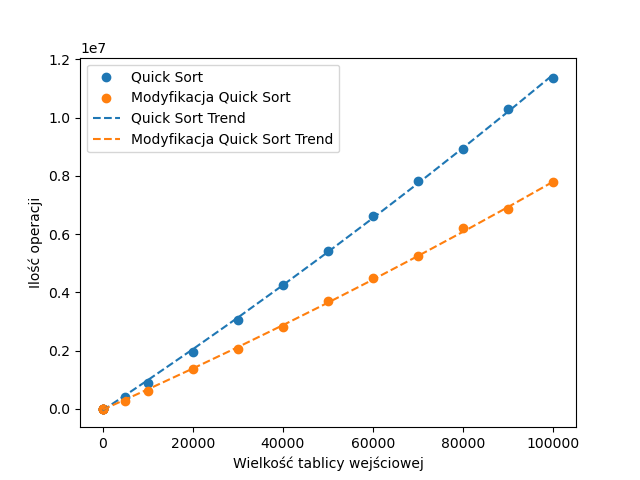
\includegraphics[width=0.8\textwidth]{Figure_1.png}
    \caption{Ilość operacji w zależności od rozmiarów tablicy wejściowej}
    \label{fig:quicksort}
\end{figure}
\begin{figure}[H]
    \centering
    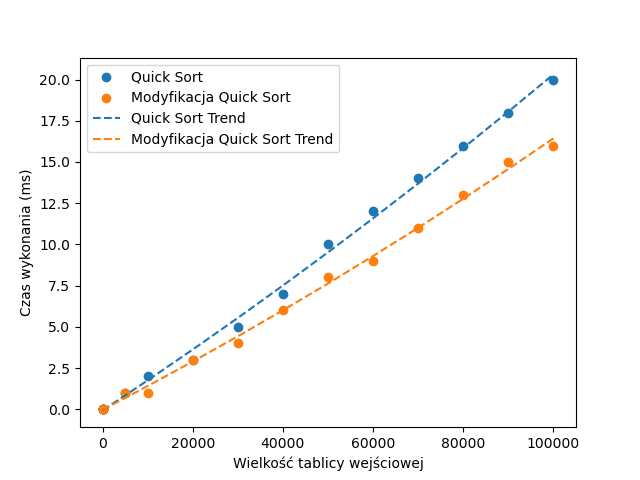
\includegraphics[width=0.8\textwidth]{Figure_2.png}
    \caption{Czas wykonania algorytmów w zależności od rozmiarów tablicy wejściowej}
    \label{fig:quicksortt}
\end{figure}
\begin{figure}[H]
    \centering
    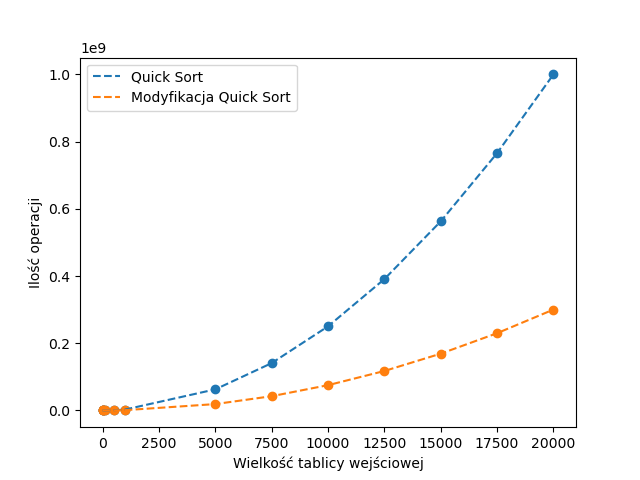
\includegraphics[width=0.8\textwidth]{Figure_7.png}
    \caption{Ilość operacji algorytmu w zależności od rozmiarów tablicy wejściowej w pesymistycznym przypadku}
    \label{fig:quicksortp}
    \begin{figure}[H]
    \centering
    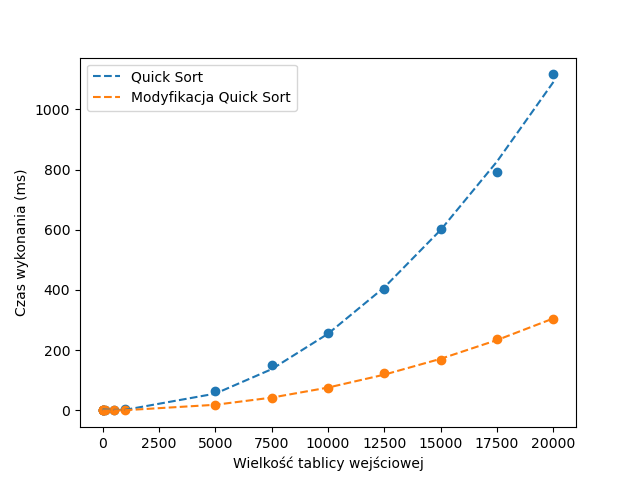
\includegraphics[width=0.8\textwidth]{Figure_8.png}
    \caption{Czas wykonania algorytmów w zależności od rozmiarów tablicy wejściowej w pesymistycznym przypadku}
    \label{fig:quicksorttp}
\end{figure}
\end{figure}
\subsection{Radix Sort}
\textit{Radix Sort} to algorytm sortowania, który należy do grupy algorytmów nieopierających się na porównaniach. Jego działanie polega na porządkowaniu liczb na podstawie kolejnych cyfr w danym systemie liczbowym, zaczynając od najmniej, a kończąc na najbardziej znaczącej pozycji. Z tego względu algorytm ten jest stosowany przy założeniu, że sortujemy tablice liczb naturalnych. Złożoność czasowa algorytmu wynosi $\Theta(k(n + d))$, gdzie:
\begin{itemize}
    \item $k$ to maksymalna liczba pozycji (cyfr) w liczbach,
    \item $n$ to liczba elementów w tablicy,
    \item $d$ to liczba różnych cyfr w systemie liczbowym (np. w systemie dziesiętnym $d = 10$).
\end{itemize}
W naszej implementacji \textit{Radix Sort} korzystamy z algorytmu \textit{Counting Sort} do sortowania elementów na podstawie każdej cyfry. Dzięki stabilności \textit{Counting Sort}, algorytm \textit{Radix Sort} jest również stabilny. Poniżej przedstawiamy jego implementację oraz opis:
\begin{lstlisting}[style=mystyle, language=C++, caption={Implementacja \texttt{Counting Sort}}, label={lst:countingsort}]
void countingSort(int A[], int n, int d, int base)
{
  int C[d];
  int B[n];
  for (int j = 0; j < d; ++j)
  {
    C[j] = 0;
  }
  for (int i = 0; i < n; ++i)
  {
    ++C[(A[i] / base) % d];
  }
  for (int j = 1; j < d; ++j)
  {
    C[j] += C[j - 1];
  }
  for (int i = n - 1; i > -1; --i)
  {
    int digit = (A[i] / base) % d;
    B[C[digit] - 1] = A[i];
    --C[digit];
  }
  for (int i = 0; i < n; ++i)
  {
    A[i] = B[i];
  }
}
\end{lstlisting}
W ogólnej formie algorytm \texttt{Counting Sort} działa poprzez zliczanie wystąpień poszczególnych liczb w tablicy $C$, a następnie obliczenie sum prefiksowych, które reprezentują ostatni indeks, na którym może znaleźć się dana liczba. Następnie, iterując od tyłu po tablicy $A$, możemy stabilnie posortować elementy, przypisując je do tablicy $B$ w odpowiednie miejsca wskazane przez tablicę $C$. 

W powyższej implementacji algorytm został dostosowany do sortowania kolejnych cyfr w $d$-arnej reprezentacji liczb, dzięki zastosowaniu parametrów $d$ oraz \texttt{base}. Dowolną liczbę $x$ w $d$-arnej reprezentacji można zapisać jako sumę:
\[
    x = \sum_{p=0}^{k} a_p d^p,
\]
gdzie $a_p \in \{0, \ldots, d-1\}$. 

Wtedy poprzez dzielenie całkowite oraz operację modulo:
\[
    \frac{x}{d^p} \mod d,
\]
możemy wyłuskać $p$-tą cyfrę w $d$-arnej reprezentacji liczby.

Teraz możemy przedstawić kod implementacji algorytmu \texttt{Radix Sort}:
\begin{lstlisting}[style=mystyle, language=C++, caption={Implementacja \texttt{Radix Sort}}, label={lst:radixsort}]
void radixSort(int A[], int n, int d)
{
  if (n == 0)
  {
    return;
  }
  int max = maximumNumber(A, n);
  for (int base = 1; max / base > 0; base *= d)
  {
    countingSort(A, n, d, base);
  }
}
\end{lstlisting}
Algorytm ten najpierw znajduje największą liczbę $max$ w tablicy $A$, a następnie iteruje przez wszystkie potęgi $d$, które występują w zapisie $max$. W każdej iteracji sortuje liczby w tablicy $A$ według kolejnych cyfr w $d$-arnym zapisie liczbowym, korzystając z algorytmu \texttt{Counting Sort}.
\subsubsection{Rozszerzenie algorytmu Radix Sort}
Powyższy algorytm można łatwo rozszerzyć na tablice liczb całkowitych. Poniżej przedstawiamy szczegóły implementacji rozszerzonej wersji \texttt{Radix Sort}:
\newpage
\begin{lstlisting}[style=mystyle, language=C++, caption={Implementacja rozszerzonej wersji \texttt{Radix Sort}}, label={lst:radixsort2}]
void negativeRadixSort(int A[], int n, int d)
{
  int positive[n];
  int negative[n];
  int p = 0;
  int neg = 0;
  for (int i = 0; i < n; ++i) {
    if (A[i] >= 0) {
      positive[p] = A[i];
      ++p;
    }
    else {
      negative[neg] = -A[i];
      ++neg;
    }
  }
  radixSort(positive, p, d);
  radixSort(negative, neg, d);
  int index = 0;
  for (int i = neg - 1; i > -1; --i) {
    A[index] = -negative[i];
    ++index;
  }
  for (int i = 0; i < p; ++i) {
    A[index] = positive[i];
    ++index;
  }
}
\end{lstlisting}

Rozszerzenie algorytmu \texttt{Radix Sort} polega na rozdzieleniu tablicy $A$ na dwie części:
\begin{itemize}
    \item tablicę wartości nieujemnych $positive$, zawierającą wszystkie liczby $\geq 0$ z tablicy $A$,
    \item tablicę modułów wartości ujemnych $negative$, zawierającą wartości $|x|$, gdzie $x < 0$.
\end{itemize}

Następnie wykonywane są następujące kroki:
\begin{enumerate}
    \item Tablica $positive$ jest sortowana przy użyciu standardowego algorytmu \texttt{Radix Sort}.
    \item Tablica $negative$ jest sortowana również algorytmem \texttt{Radix Sort}.
    \item Tablica posortowana jest tworzona poprzez połączenie odwróconej tablicy $negative$ (z powrotem jako liczby ujemne) z tablicą $positive$.
\end{enumerate}

Dzięki temu podejściu algorytm może efektywnie i stabilnie sortować zarówno liczby dodatnie, jak i ujemne.

\subsubsection{Wyniki dla Radix Sort}
Tabele poniżej przedstawiają wyniki eksperymentów dla algorytmu \textit{Radix Sort} względem różnych podstaw $d$:
\begin{table}[H]
    \centering
    \scalebox{0.9}{
    \begin{tabular}{|c|c|c|c|c|c|c|}
    \hline
    \textbf{Wielkość tablicy} & \textbf{$d=2$} & \textbf{$d=10$} & \textbf{$d=16$} & \textbf{$d=256$} & \textbf{$d=1024$} & \textbf{$d=16384$} \\ \hline
    \textbf{5} & 2,018 & 1,247 & 1,414 & 9,064 & 23,580 & 373,788 \\ \hline
    \textbf{10} & 3,255 & 1,653 & 1,762 & 9,753 & 24,982 & 393,622 \\ \hline
    \textbf{100} & 24,147 & 8,678 & 7,797 & 13,808 & 28,046 & 396,688\\ \hline
    \textbf{5,005} & 1,162,114 & 391,277 & 336,441 & 234,542 & 194,825 & 563,465 \\ \hline
    \textbf{10,000} & 2,320,954 & 780,888 & 671,106 & 459,318 & 364,654 & 733,297 \\ \hline
    \textbf{50,005} & 11,602,117 & 3,928,768 & 3,351,442 & 2,259,543 & 1,724,830 & 2,093,470 \\ \hline
    \textbf{80,000} & 18,560,960 & 6,328,616 & 5,361,108 & 3,609,319 & 2,744,659 & 3,113,298 \\ \hline
    \textbf{100,000} & 23,200,960 & 7,911,114 & 6,701,111 & 4,509,323 & 3,424,662 & 3,793,299 \\ \hline
    \end{tabular}
    }
    \caption{Liczba operacji dla algorytmu \texttt{Radix Sort} przy podstawie $d$ w zależności od rozmiarów tablicy wejściowej}
    \label{tab:radixsort_results}
\end{table}

\begin{table}[H]
    \centering
    \scalebox{0.9}{
    \begin{tabular}{|c|c|c|c|c|c|c|}
    \hline
    \textbf{Wielkość tablicy} & \textbf{$d=2$} & \textbf{$d=10$} & \textbf{$d=16$} & \textbf{$d=256$} & \textbf{$d=1024$} & \textbf{$d=16384$} \\ \hline
    \textbf{5} & 0 & 0 & 0 & 0 & 0 & 1 \\ \hline
    \textbf{10} & 0 & 0 & 0 & 0 & 0 & 1 \\ \hline
    \textbf{100} & 0 & 0 & 0 & 0 & 0 & 1 \\ \hline
    \textbf{5,005} & 3 & 1 & 1 & 1 & 1 & 1 \\ \hline
    \textbf{10,000} & 6 & 2 & 2 & 2 & 1 & 1\\ \hline
    \textbf{50,005} & 38 & 11 & 9 & 6 & 4 & 5 \\ \hline
    \textbf{80,000} & 47 & 18 & 13 & 10 & 7 & 8 \\ \hline
    \textbf{100,000} & 61 & 23 & 19 & 12 & 9 & 10 \\ \hline
    \end{tabular}
    }
    \caption{Czas wykonywania(ms) dla algorytmu \texttt{Radix Sort} przy podstawie $d$ w zależności od rozmiarów tablicy wejściowej}
    \label{tab:radixsortt_results}
\end{table}

Z tabel wynika, że zwiększanie wartości $d$ przynosi wymierne korzyści w przypadku dużych tablic, jednak dla małych tablic powoduje wydłużenie czasu działania algorytmu.

\begin{figure}[H]
    \centering
    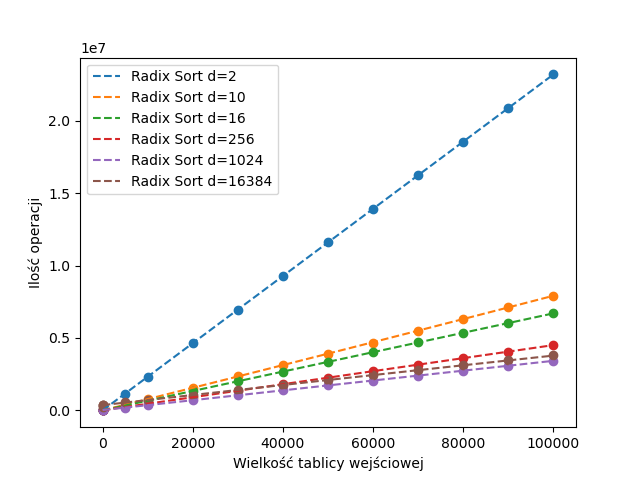
\includegraphics[width=0.8\textwidth]{Figure_3.png}
    \caption{Ilość operacji w zależności od rozmiarów tablicy wejściowej i podstawy $d$}
    \label{fig:radixsort}
\end{figure}
\begin{figure}[H]
    \centering
    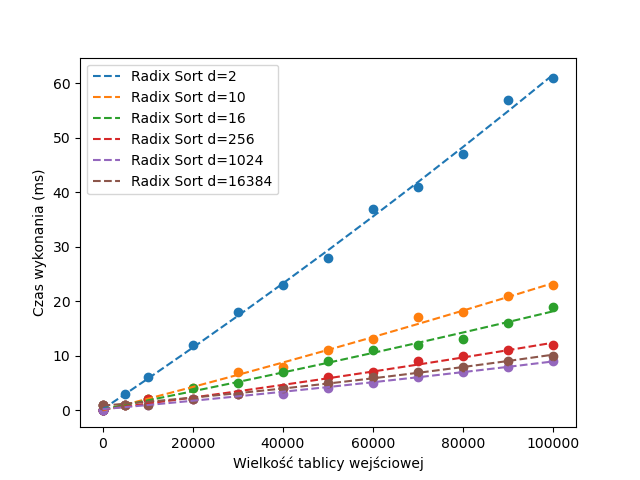
\includegraphics[width=0.8\textwidth]{Figure_4.png}
    \caption{Czas działania algorytmu (ms) w zależności od rozmiarów tablicy wejściowej i bazy $d$}
    \label{fig:radixsortt}
\end{figure}
\subsection{Bucket Sort}
\textit{Bucket Sort} to algorytm sortowania, który opiera się na podziale danych na mniejsze grupy, zwane \textit{kubełkami} (ang. \textit{buckets}), a następnie posortowaniu każdego kubełka osobno. W zależności od algorytmu użytego do sortowania zawartości kubełków, \textit{Bucket Sort} ma pesymistyczną złożoność czasową $\bigO(n^2)$ lub $\bigO(n \log n)$. Popularność tego algorytmu wynika z faktu, że przy założeniu, iż sortujemy liczby z przedziału $(0, 1]$, rozłożone jednostajnie na tym przedziale, średnia złożoność czasowa wynosi $\Theta(n)$. Kluczową rolę w implementacji algorytmu \textit{Bucket Sort} pełni struktura listy, której najważniejszą część przedstawiamy poniżej:
\begin{lstlisting}[style=mystyle, language=C++, caption={Implementacja \texttt{Listy}}, label={lst:list}]
struct Node {
  Node *prev = nullptr;
  double key;
  Node *next = nullptr;
};
struct List {
  Node *head = nullptr;
};
\end{lstlisting}
Struktura ta składa się z węzłów, które są połączone za pomocą wskaźników wskazujących na poprzedni oraz następny element listy. Często implementuje się razem z listą metody \textbf{INSERT}, \textbf{DELETE} oraz \textbf{SEARCH}. Pierwsza z nich jest wykorzystywana w implementacji algorytmu \textit{Bucket Sort}, dlatego jej implementacja została przedstawiona poniżej:

\begin{lstlisting}[style=mystyle, language=C++, caption={Implementacja \texttt{Insert}}, label={lst:list_insert}]
void insert(Node *x)
{
  x->next = this->head;
  x->prev = nullptr;
  if (this->head == nullptr)
  {
    this->head = x;
  }
  else
  {
    this->head->prev = x;
    this->head = x;
  }
}
\end{lstlisting}
Metoda ta wstawia nowy węzeł na początek listy oraz aktualizuje wskaźnik na \textbf{HEAD}. Bardzo ważnym elementem algorytmu \textit{Bucket Sort} jest również możliwość sortowania listy. Można to przeprowadzić na dwa sposoby: sortując całą listę po wstawieniu wszystkich elementów lub sortując listę na bieżąco, podczas dodawania każdego elementu. W tej implementacji algorytmu \textit{Bucket Sort} zastosowaliśmy algorytm \textit{Insertion Sort}. Zdecydowaliśmy się na sortowanie na bieżąco, dlatego poniżej przedstawiamy zmieniony kod metody \textbf{INSERT}. Dla zainteresowanych, alternatywna wersja sortowania całej listy została zaimplementowana w pliku \textit{list.cpp}.
\newpage
\begin{lstlisting}[style=mystyle, language=C++, caption={Implementacja \texttt{Insert} z sortowaniem}, label={lst:insert2}]
void insert(Node *x)
{
  if (this->head == nullptr)
  {
    this->head = x;
    return;
  }
  Node *curr = this->head;
  if (curr->key >= x->key)
  {
    x->next = this->head;
    this->head->prev = x;
    x->prev = nullptr;
    this->head = x;
    return;
  }
  while (curr->next != nullptr && curr->next->key < x->key)
  {
    curr = curr->next;
  }
  if (curr->next == nullptr)
  {
    curr->next = x;
    x->prev = curr;
    x->next = nullptr;
  }
  else
  {
    x->next = curr->next;
    x->prev = curr;
    curr->next->prev = x;
    curr->next = x;
  }
}
\end{lstlisting}
Nowa wersja metody \textbf{INSERT} na początku oddzielnie rozpatruje przypadki, gdy lista jest pusta lub gdy nowy węzeł musi zostać wstawiony na początek listy. Jeśli te przypadki nie zachodzą, metoda szuka miejsca, w które nowy węzeł powinien zostać wstawiony. Następnie wstawia nowy węzeł w odpowiednie miejsce, w zależności od tego, czy jest to koniec, czy środek listy, wykonując odpowiednie operacje i aktualizując wskaźniki.

Teraz możemy przedstawić finalną implementację algorytmu \textit{Bucket Sort}. W implementacji uwzględniliśmy dodatkową modyfikację, która umożliwia sortowanie na dowolnym przedziale liczbowym, a nie tylko na przedziale $(0, 1]$. Osiągnęliśmy to dzięki zastosowaniu normalizacji min-max, czyli przekształcenia danych za pomocą wzoru:
\[
    x' = \frac{x - \min(x)}{\max(x) - \min(x)}
\]
gdzie $x$ to wartość oryginalna, a $x'$ to wartość znormalizowana, która mieści się w przedziale $[0, 1]$.
\newpage
\begin{lstlisting}[style=mystyle, language=C++, caption={Implementacja \texttt{Bucket Sort}}, label={lst:bucketsort}]
void bucketSort(double A[], int n)
{
  if (n == 0)
  {
    return;
  }
  Pair maxmin = maxminNumber(A, n);
  double min = maxmin.first;
  double max = maxmin.second;
  if (max == min)
  {
    return;
  }
  int range = max - min;
  List *B[n];
  for (int i = 0; i < n + 1; ++i)
  {
    B[i] = new List;
  }
  for (int i = 0; i < n; ++i)
  {
    Node *element = new Node;
    element->key = A[i];
    int index = int((element->key - min) / range * n);
    if (index == n)
    {
      --index;
    }
    B[index]->insert(element);
  }
  int idx = 0;
  for (int i = 0; i < n; ++i)
  {
    Node *curr = B[i]->head;
    while (curr != nullptr)
    {
      A[idx] = curr->key;
      ++idx;
      curr = curr->next;
    }
  }
}
\end{lstlisting}

W pierwszym kroku algorytmu \textit{Bucket Sort} znajdujemy najmniejszą i największą liczbę w tablicy $A$. Następnie tworzymy tablicę kubełków $B$ o rozmiarze równym liczbie elementów w tablicy $A$, a każdemu kubełkowi przypisujemy listę, która będzie pełniła rolę kubełka.

Następnie, iterując po tablicy $A$, przypisujemy każdy element do odpowiedniego kubełka. Indeks kubełka, do którego trafi dany element, obliczany jest na podstawie znormalizowanej wartości elementu, którą uzyskujemy poprzez obliczenie różnicy między wartością elementu a minimalną wartością w tablicy, a następnie przemnożenie tej różnicy przez $n$ (liczba elementów w tablicy). W przypadku, gdy obliczony indeks odpowiada najwyższemu możliwemu indeksowi w tablicy kubełków, stosujemy specjalny warunek, aby uniknąć przekroczenia zakresu tablicy. Warto wspomnieć, że wstawiany element jest automatycznie sortowany dzięki zastosowaniu algorytmu wstawiania przedstawionego wyżej.

Na końcu algorytmu, iterując po wszystkich kubełkach w tablicy $B$, wyciągamy elementy z poszczególnych list i wstawiamy je z powrotem do tablicy $A$. Po tej operacji tablica $A$ będzie posortowana.

\subsubsection{Wyniki dla Bucket Sort}
Tabele poniżej przedstawiają wyniki eksperymentów dla algorytmu \textit{Bucket Sort}:
\begin{table}[H]
    \centering
    \scalebox{0.9}{
    \begin{tabular}{|c|c|c|c|c|}
    \hline
    \textbf{Wielkość tablicy} & \textbf{Ilość przypisań} & \textbf{Ilość porównań} & \textbf{Łączna liczba operacji} & \textbf{Czas (ms)} \\ \hline
    \textbf{5} & 91 & 79 & 170 & 0 \\ \hline
    \textbf{10} & 167 & 153 & 320 & 0 \\ \hline
    \textbf{100} & 1,582 & 1,518 & 3,100 & 0 \\ \hline
    \textbf{5,005} & 78,101 & 75,400 & 153,501 & 1 \\ \hline
    \textbf{10,000} & 156,168 & 150,793 & 306,961 & 2 \\ \hline
    \textbf{50,005} & 780,305 & 753,587 & 1,533,892 & 11 \\ \hline
    \textbf{80,000} & 1,248,346 & 1,205,677 & 2,454,023 & 25 \\ \hline
    \textbf{100,000} & 1,560,435 & 1,507,203 & 3,067,638 & 34 \\ \hline
    \end{tabular}
    }
    \caption{Liczba operacji i czas wykonania dla algorytmu \texttt{Bucket Sort} przy różnych rozmiarach tablicy}
    \label{tab:bucketsort_results}
\end{table}
\begin{table}[H]
    \centering
    \scalebox{0.9}{
    \begin{tabular}{|c|c|c|c|c|}
    \hline
    \textbf{Wielkość tablicy} & \textbf{Ilość przypisań} & \textbf{Ilość porównań} & \textbf{Łączna liczba operacji} & \textbf{Czas (ms)} \\ \hline
    \textbf{5} & 100 & 90 & 190 & 0 \\ \hline
    \textbf{10} & 220 & 206 & 426 & 0 \\ \hline
    \textbf{100} & 6,568 & 6,466 & 13,034 & 0 \\ \hline
    \textbf{5,005} & 12,617,577 & 12,612,573 & 25,230,150 & 37 \\ \hline
    \textbf{10,000} & 50,213,876 & 50,203,879 & 100,417,755 & 139 \\ \hline
    \textbf{20,005} & 200,584,455 & 200,564,459 & 401,148,914 & 606 \\ \hline
    \end{tabular}
    }
    \caption{Liczba operacji i czas wykonania dla algorytmu \texttt{Bucket Sort} przy różnych rozmiarach tablicy w pesymistycznym przypadku}
    \label{tab:bucketsortp_results}
\end{table}

Poniżej przedstawiamy wykresy, na których porównujemy algorytm \textit{Bucket Sort} z algorytmem \textit{Quick Sort}.

\begin{figure}[H]
    \centering
    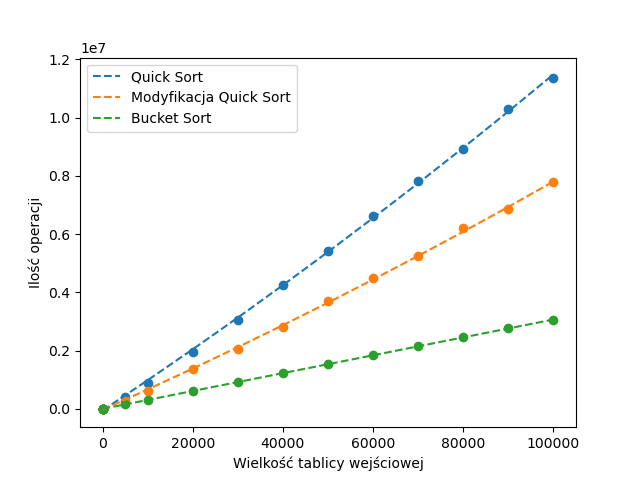
\includegraphics[width=0.8\textwidth]{Figure_5.png}
    \caption{Ilość operacji w zależności od rozmiarów tablicy wejściowej}
    \label{fig:bucket}
\end{figure}
\begin{figure}[H]
    \centering
    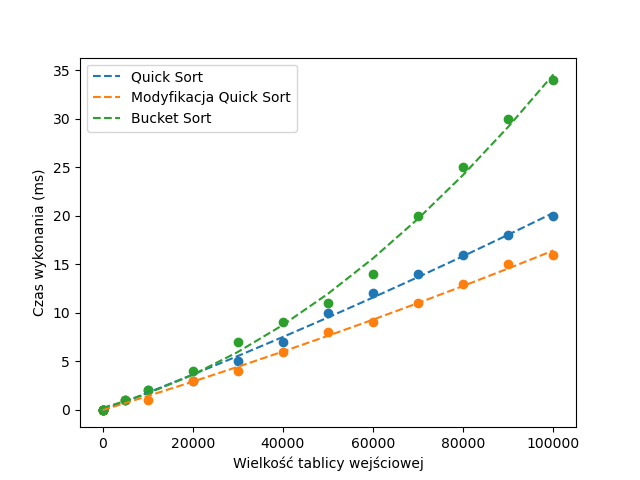
\includegraphics[width=0.8\textwidth]{Figure_6.png}
    \caption{Czas działania algorytmów w zależności od rozmiarów tablicy wejściowej}
    \label{fig:buckett}
\end{figure}
\begin{figure}[H]
    \centering
    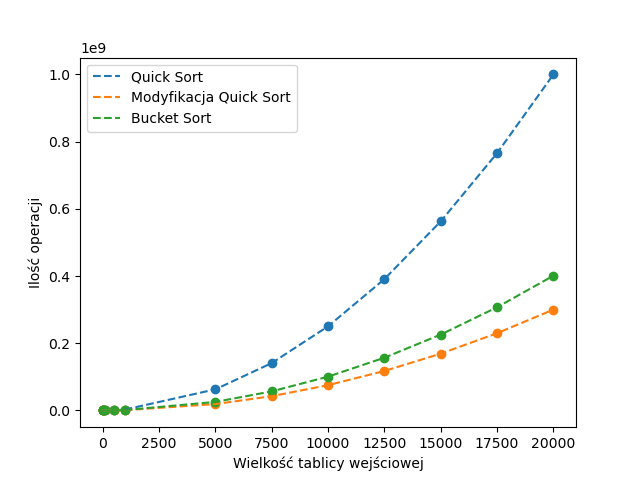
\includegraphics[width=0.8\textwidth]{Figure_9.png}
    \caption{Ilość operacji w zależności od rozmiarów tablicy wejściowej w pesymistycznym przypadku}
    \label{fig:bucket}
\end{figure}
\begin{figure}[H]
    \centering
    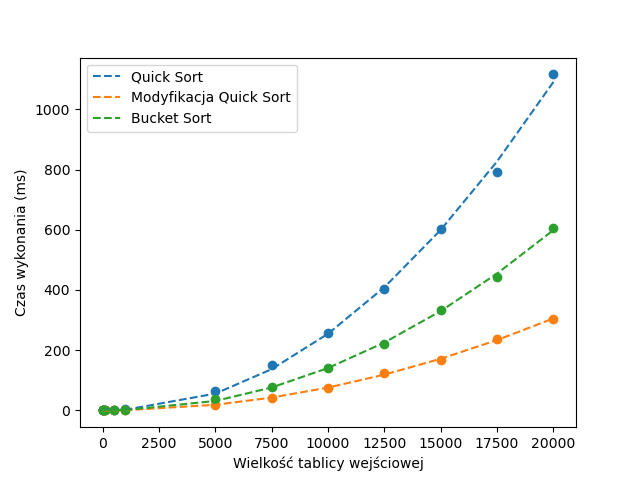
\includegraphics[width=0.8\textwidth]{Figure_10.png}
    \caption{Czas działania algorytmów w zależności od rozmiarów tablicy wejściowej}
    \label{fig:buckett}
\end{figure}
Co ciekawe, pomimo mniejszej liczby operacji wykonywanych przez algorytm \texttt{Bucket Sort}, jego czas działania jest zauważalnie dłuższy. Wynika to z faktu, że tworzenie list oraz wykonywanie na nich operacji jest znacznie wolniejsze niż przeprowadzanie tych samych operacji na tablicach. Teoretycznym usprawnieniem mogłoby być zmniejszenie liczby kubełków.
\section{Wnioski}
Z przeprowadzonej analizy wynika, że wybór algorytmu sortującego zależy głównie od charakterystyki danych wejściowych oraz ich rozmiaru. W ogólnym przypadku (bez dodatkowych założeń) algorytm \texttt{Quick Sort} jest najczęściej najlepszym wyborem ze względu na swoją elastyczność (może posortować praktycznie każdy rodzaj danych) oraz bardzo dobrą średnią złożoność czasową $\bigO(n \log n)$. 

W sytuacjach, gdy dane wejściowe są liczbami całkowitymi, algorytm \texttt{Radix Sort} wykazuje znacznie lepszą wydajność, szczególnie gdy wybór odpowiedniej podstawy $d$ jest dopasowany do specyfiki danych. \texttt{Radix Sort}, przy odpowiednich założeniach, jest algorytmem o złożoności liniowej, co czyni go niezwykle efektywnym, zwłaszcza dla dużych zbiorów danych. Jego skuteczność zależy jednak w dużej mierze od właściwego dobrania podstawy $d$, co może wymagać dodatkowej analizy.

Z kolei, jeśli dodatkowym założeniem jest jednostajny rozkład liczb w zadanym przedziale, bardzo dobrą efektywność wykazuje algorytm \texttt{Bucket Sort}. Jego złożoność czasowa jest zależna od liczby kubełków oraz rozkładu danych pomiędzy tymi kubełkami. Sprawdza się on szczególnie dobrze, gdy dane są równomiernie rozmieszczone. Dla danych rozproszonych w szerokim przedziale, \texttt{Bucket Sort} może znacząco poprawić wydajność sortowania. Niemniej, posiada on istotną wadę — operacje na listach są znacznie wolniejsze niż operacje na tablicach, co może negatywnie wpływać na czas działania algorytmu.

Podsumowując, decyzja o wyborze algorytmu sortującego powinna być oparta na analizie charakterystyki danych. W wielu przypadkach odpowiedni dobór algorytmu pozwala na znaczną optymalizację procesu sortowania, co prowadzi do zmniejszenia złożoności obliczeniowej problemu.
\end{document}
